\باب{بنیادی حقائق}
اس کتاب میں جگہ جگہ مختلف حقائق آئیں گے جنہیں اس باب میں اکٹھے کرنے کی کوشش کی گئی ہے۔یہ توقع کی جاتی ہے کہ یوں کتاب پڑھتے وقت اصل مضمون پر توجہ رکھنا زیادہ آسان ہوگا۔

\حصہ{بنیادی اکائیاں}
اس کتاب میں  \اصطلاح{بین الاقوامی نظامِ اکائی}\حاشیہب{International System Of Units, SI} استعمال کیا جائے گا۔ اس نظام میں کمیت\حاشیہب{mass} کی اکائی \اصطلاح{کلوگرام}،  لمبائ کی اکائی \اصطلاح{میٹر} اور وقت کی اکائی \اصطلاح{سیکنڈ} ہے۔

\حصہ{مقداری}
وہ متغیرہ جس کی مقدار معین ہو اسے \اصطلاح{مقداری}\فرہنگ{مقداری}\حاشیہب{scalar}\فرہنگ{scalar} کہتے ہیں۔ اس کتاب میں مقداری متغیرہ کو سادہ طرز کی لکھائی میں انگریزی یا لاطینی زبان کے چھوٹے حروف  یعنی \عددی{a,b,\alpha,\cdots}  یا بڑے حروف یعنی  \عددی{A,B,\Psi,\cdots} سے ظاہر کیا جائے گا، مثلاً برقی رو کو \عددی{i} یا \عددی{I} سے ظاہر کیا جاتا ہے۔

\حصہ{سمتیہ}
	وہ خط جس کا طول اور سمت معین ہو، اسے \اصطلاح{سمتیہ}\فرہنگ{سمتیہ}\حاشیہب{vector}\فرہنگ{vector} کہتے ہیں۔ سمتیہ کو انگریزی یا لاطینی زبان کے چھوٹے یا  بڑے حروف،  جن کو موٹے طرز کی لکھائی میں لکھا گیا ہو،  سے ظاہر کیا جائے گا، مثلاً قوت کو \سمتیہ{F} سے ظاہر کیا جائے گا۔یہاں شکل \حوالہ{شکل_حقائق_اکائی_سمتیہ}  سے رجوع کرنا بہتر ہے۔ ایک ایسا سمتیہ جس کا طول ایک کے برابر ہو،  کو \اصطلاح{اکائی سمتیہ}\فرہنگ{اکائی سمتیہ}\حاشیہب{unit vector}\فرہنگ{unit vector} کہتے ہیں۔ اس کتاب میں اکائی سمتیہ کو انگریزی زبان کے پہلے حرف کو موٹے طرز کی لکھائ میں لکھا جائے گا، مثلاً اکائی سمتیہ \عددیء{\ax,\ay,\az} خلاء کی تین عمودی سمتوں کو ظاہر کرتے ہیں۔\عددیء{\ax} لکھتے ہوئے، زیرنوشت میں \عددیء{x}، اس بات کی نشان دہی  کرتا ہے کہ یہ اکائی سمتیہ خلاء کی \عددیء{x} سمت کو ظاہر کرتا ہے۔ اگر کسی سمتیہ  کا طول اور اس کی سمت کو علیحدہ علیحدہ لکھنا ہو تو اس کے طول کو ظاہر کرنے کے لئے سادہ طرز کی لکھائی میں وہی حرف استعمال کیا جائے گا جو اس سمتیہ کو ظاہر کرنے کے لئے، موٹے طرز کی لکھائی میں، استعمال کیا گیا ہو۔ یعنی سمتیہ \سمتیہ{F} کے طول کو \عددیء{F} سے ظاہر کیا جائے گا۔ شکل میں سمتیہ  \سمتیہ{F} کا طول \عددیء{F}، چار کے برابر ہے۔ اگر کسی سمتیہ کی سمت میں ایک اکائی سمتیہ بنایا جائے تو یہ اکائی سمتیہ اس سمتیہ کی سمت کو ظاہر کرتا ہے۔جیسے پہلے ذکر ہوا ہے  ایسے اکائی سمتیہ کو انگریزی کے پہلے حرف،  جس کو موٹے طرز کی لکھائی میں لکھا گیا ہو  سے ظاہر کیا جائے گا یعنی سمتیہ \سمتیہ{F} کی سمت کو \عددیء{\سمتیہ{a}_F} سے ظاہر کیا جائے گا۔یہاں،  زیرنوشت میں \عددیء{F} ، اس بات کی یاد دہانی کراتا ہے کہ یہ اکائی سمتیہ \سمتیہ{F} کی سمت کو ظاہر کر رہا ہے۔ شکل میں چونکہ قوت \سمتیہ{F} کا رخ دائیں جانب ہے لہٰذا  \عددیء{\سمتیہ{a}_F} اور  \عددیء{\ax} برابر ہیں۔
\begin{figure}
\centering
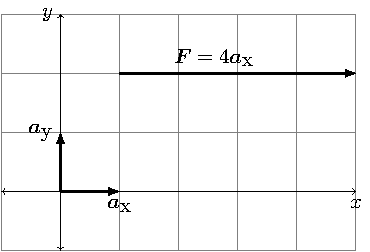
\includegraphics{figBasicFactsUnitVectors}
\caption{کارتیسی محدد}
\label{شکل_حقائق_اکائی_سمتیہ}
\end{figure}
%
\حصہ{محدد، خط مرتب}
ایک ایسا طریقہ جس کے ذریعہ کسی نقطہ کا مقام متعین کیا جا سکے کو خط مرتب یا محدد کہتے ہیں۔

	 خلاء تین طرفہ ہے۔ لہٰذا اس میں کسی ایک نقطہ کے مقام کو تین محدد کی مدد سے ظاہر کیا جا سکتا ہے۔ مزید یہ کہ خلاء میں کسی سمتیہ کو تین عمودی اکائی سمتیوں کی مدد سے لکھا جا سکتا ہے۔اب ہم ایسے چند محدد کے نظام دیکھتے ہیں۔

\جزوحصہ{کارتیسی محدد کا نظام}
	شکل \حوالہ{شکل_حقائق_اکائی_سمتیہ}   میں خلاء کی دو سمتیں اکائی سمتیہ \عددیء{\ax} اور \عددیء{\ay} سے ظاہر کی گئی ہیں۔یہ دونوں  آپس میں عمودی ہیں یعنی ان کا آپس میں \عددیء{90\degree}  کا زاویہ ہے۔خلاء تین طرفہ ہے لہٰذا اسے تین \اصطلاح{عمودی اکائی سمتیات}\فرہنگ{سمتیہ!عمودی اکائی}\حاشیہب{orthonormal vectors}\فرہنگ{orthonormal} سے ظاہر کیا جاتا ہے۔ ان سمتوں کی جانب،  طول  کو \عددیء{x,y,z} سے ظاہر کیا جاتا ہے۔ آپ ان سے بخوبی واقف ہیں۔ 


	 اگر دائیں ہاتھ کی چار انگلیوں کو \عددیء{\ax} کی جانب رکھ کر انہیں \عددیء{\ay} کی جانب موڑا جائے تو اس ہاتھ کا انگوٹھا \عددیء{\az} کی سمت کو ظاہر کرے گا۔لہٰذا،  خلاء کا  یہ  تین اکائی سمتوں والا نظام ایک \اصطلاح{دائیں ہاتھ کا نظام}\حاشیہب{right handed coordinate system}  ہے۔

	شکل \حوالہ{شکل_حقائق_کارتیسی_نظام_ایک_سمتیہ}  میں ایک سمتیہ \سمتیہ{A}، مرکز سے نقطہ \عددی{P(x,y,z)} تک بنایا گیا ہے۔اس سمتیہ کو ہم کارتیسی نظام محدد میں تین سمتیہ سے یوں ظاہر کر سکتے ہیں۔
\begin{align}
\kvec{A}=\kvec{A}_x+\kvec{A}_y+\kvec{A}_z
\end{align}
یا
\begin{align}
\kvec{A}=x\ax+y\ay+z\az
\end{align}
%
\begin{figure}
\centering
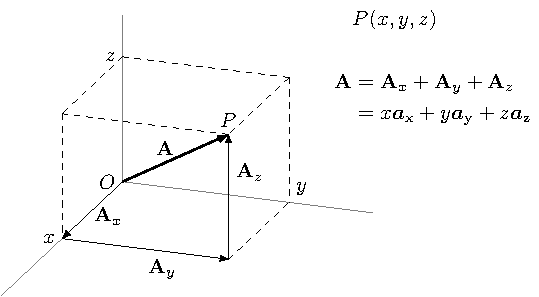
\includegraphics{figBasicFactsVectorCartesianCoordinates}
\caption{کارتیسی محدد نظام میں ایک سمتیہ}
\label{شکل_حقائق_کارتیسی_نظام_ایک_سمتیہ}
\end{figure}
%
کارتیسی محدد کے نظام میں اگر ہم متغیرہ \عددی{z} کو صفر رکھیں اور \عددیء{x,y} کو تبدیل کریں تو ہمیں  سطح \عددی{x-y} ملتی ہے۔ اس طرح اگر شکل \حوالہ{شکل_حقائق_کارتیسی_نظام_ایک_سمتیہ}  میں نقطہ \عددی{P(2,4,3)} ہو اور \عددیء{x-y} سطح کو زمین سمجھا جائے  تو شکل میں ڈبہ کے بالائی سطح پر  \عددی{z} کی مقدار معین ہے یعنی  \عددیء{z=3} جبکہ \عددی{x} صفر سے تین کے درمیان تبدیل اور \عددی{y} صفر سے چار کے درمیان تبدیل ہوتا ہے۔ یعنی اس ڈبہ کے بالائی سطح کو یوں لکھا جا سکتا ہے۔ 
\begin{align}
 \text{ڈبے کا بالائی سطح}= \left\{ 
  \begin{array}{l}
    0<x<2\\
    0<y<4 \\
	 z=3
  \end{array} \right.
\end{align}
اسی طرح اگر \عددیء{z} کو صفر اور تین کے درمیان ہر ممکن قیمت پر رکھ کر \عددی{x} اور \عددی{y} کو اسی طرح ان حدوں کے درمیان تبدیل کیا جائے تو ہمیں اس ڈبہ کا پورا حجم حاصل ہوگا۔ لہٰذا اس ڈبہ کے حجم کو ہم یوں لکھ سکتے ہیں۔
\begin{align}
 \text{ڈبے کاحجم}= \left\{ 
  \begin{array}{l}
    0<x<2\\
    0<y<4 \\
    0<z<3
  \end{array} \right.
\end{align}

\جزوحصہ{نلکی محدد کا نظام}
شکل \حوالہ{شکل_حقائق_نلکی_نظام_ایک_سمتیہ}  میں ایک سمتیہ  \سمتیہ{A} مرکز سے نقطہ \عددیء{P(x,y,z)} تک بنایا گیا ہے۔ اس سمتیہ کو شکل میں دو سمتیوں کی مدد سے ظاہر کیا گیا ہے۔ یعنی
\begin{align}
\kvec{A}=\kvec{\rho}+\kvec{A}_z
\end{align}
یا
\begin{align}
\kvec{A}=\rho \arho+z \az
\end{align}
%
\begin{figure}
\centering
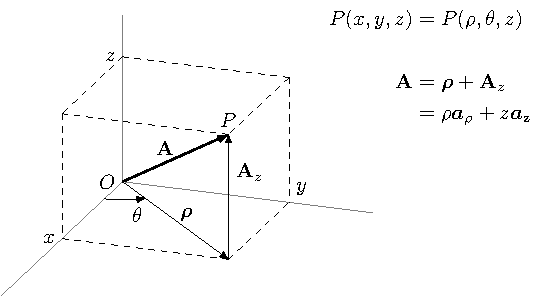
\includegraphics{figBasicFactsVectorCylindricalCoordinates}
\caption{نلکی محدد نظام}
\label{شکل_حقائق_نلکی_نظام_ایک_سمتیہ}
\end{figure}
سمتیہ $\arho$ سطح \عددی{x-y} پر ہے۔ اس شکل سے ظاہر ہے کہ
\begin{align}
x&=\rho \cos \theta\\
y&=\rho \sin \theta
\end{align}
لہٰذا ہم نقطہ \عددی{P(x,y,z)} کو متغیرہ \عددیء{x,y,z} کی جگہ متغیرہ \عددیء{\rho,\theta,z} کی مدد سے یوں لکھ سکتے ہیں \عددیء{P(\rho,\theta,z)}۔ لہٰذا ہم خلاء میں کسی بھی نقطہ کو اس کے تین متغیرہ \عددیء{\rho,\theta,z} سے ظاہر کر سکتے ہیں۔

	وہ نظام جس میں متغیرہ \عددیء{\rho,\theta,z}  کسی نقطہ کو متعین کرنے کے لئے استعمال ہو تو اس کو \اصطلاح{نلکی محدد}\فرہنگ{محدد!نلکی}\حاشیہب{cylindrical co-ordinates}\فرہنگ{cylindrical co-ordinates} کہتے ہیں۔یہاں شکل \حوالہ{شکل_حقائق_نلکی_نظام_تعریف}  سے رجوع کریں۔ اس نظام کے تین عمودی  اکائی سمتیہ $\arho,\atheta,\az$ ہیں۔ یہ نظام بھی دائیں ہاتھ کا نظام ہے۔ لہٰذا اگر دائیں ہاتھ کی چار انگلیوں کو اکائی سمتیہ $\arho$ کی جانب رکھ کر انہیں $\atheta$ کی جانب موڑیں تو اس ہاتھ کا انگوٹھا $\az$ کی سمت میں ہوگا۔ یہ تین عمودی اکائی سمتیہ کی تفصیل یوں ہے۔

سطح \عددی{x-y} میں محدد \عددی{x} سے  زاویہ \عددی{\theta} کی  جانب اگر  اکائی سمتیہ بنائی جائے تو یہ اکائی سمتیہ $\arho$ ہو گی۔ اگر اسی سطح  \عددیء{x-y} پر اکائی سمتیہ $\arho$ کی عمودی سمت میں، زاویہ  \عددی{\theta} بڑھانے والے سمت میں، ایک اکائی سمتیہ بنائی جائے تو یہ  اکائی سمتیہ $\atheta$ ہو گی۔ اکائی سمتیہ $\az$ وہی اکائی سمتیہ ہے جو کارتیسی محدد نظام میں تھی۔ 
\begin{figure}
\centering
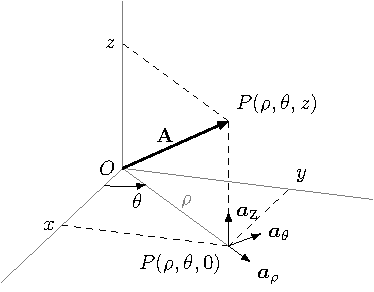
\includegraphics[height=3.5cm]{figBasicFactsCylindricalCoordinates}
\caption{نلکی نما محدد کی تعریف}
\label{شکل_حقائق_نلکی_نظام_تعریف}
\end{figure}
	یہاں یہ واضح رہے کہ اس نلکی محدد کے نظام  میں $\arho$ اور  $\atheta$ کی سمتیں ہر نقطہ پر مختلف ہیں جیسا کہ شکل \حوالہ{شکل_حقائق_نلکی_نظام_میں_اکائی_سمتیات_اٹل_نہیں} میں دکھایا گیا ہے۔

یہاں شکل \حوالہ{شکل_حقائق_نلکی_نظام_میں_دائرہ_اور_نلکی}  سے رجوع کریں۔ اگر نلکی محدد میں ایک سمتیہ ( جس کا متغیرہ \عددی{z} صفر کے برابر ہو، یعنی \عددی{z=0} ، اور اس کا رداس  \عددیء{\rho} ایک مستقل مقدار ہو مثلاً \عددیء{\rho=\rho_0}) کو یوں بنایا جائے کہ اس کا زاویہ \عددی{\theta} کو صفر سے  \عددیء{2 \pi} تک لے جایا جائے تو اس سمتیہ کی چونچ سطح \عددی{x-y} پر ایک دائرہ بنائے گی۔ اب اگر اسی سمتیہ کے متغیرہ \عددی{z} کو بھی تبدیل کیا جائے، مثلاً \عددی{z} کو صفر اور تین کے درمیان اس طرح تبدیل کیا جائے کہ ہر \عددی{\theta} پر \عددیء{z} کو صفر سے تین تک لے جایا جائے تو یہ سمتیہ ایک نلکی بنائے گی۔ اسی وجہ سے اس نظام کو نلکی محدد کہتے ہیں۔ اب اگر ہم سمتیہ کے تینوں متغیرہ تبدیل کریں تو ہمیں نلکی کا حجم ملتا ہے۔ اگلے تین مساوات ان باتوں کو ظاہر کرتے ہیں۔
\begin{align}
 \text{دائرہ}&= \left\{ 
  \begin{array}{l}
    \rho=\rho_0\\
    0<\theta<2 \pi \\
    z=0
  \end{array} \right.
\end{align}
%
\begin{align}
 \text{نلکی نما سطح}&= \left\{ 
  \begin{array}{l}
    \rho=\rho_0\\
    0<\theta<2 \pi \\
  0<z<z_0
  \end{array} \right.
\end{align}
%
\begin{align}
 \text{نلکی کا حجم}= \left\{ 
  \begin{array}{l}
    0<\rho<\rho_0\\
    0<\theta<2 \pi \\
  0<z<z_0
  \end{array} \right.
\end{align}
%
\begin{figure}
\centering
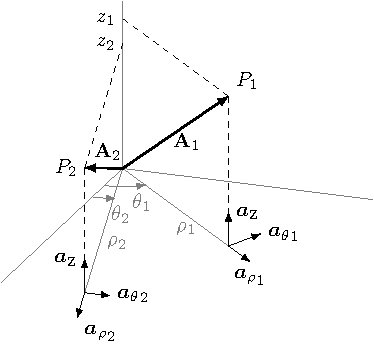
\includegraphics[height=3.5cm]{figBasicFactsCylindricalCoordinatesVaryingUnitVectors}
\caption{نلکی محدد میں اکائی سمتیہ \عددیء{\arho} اور \عددیء{\atheta} ہر نقطہ پر مختلف ہیں۔}
\label{شکل_حقائق_نلکی_نظام_میں_اکائی_سمتیات_اٹل_نہیں}
\end{figure}
%
\begin{figure}
\centering
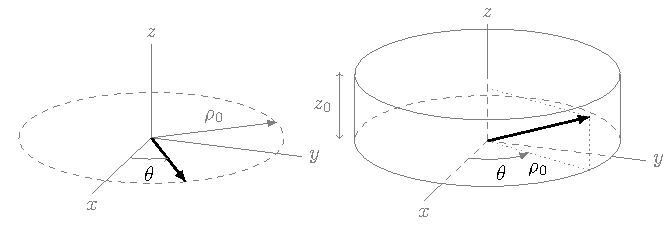
\includegraphics[height=2.5cm]{figBasicFactsCylindricalCoordinatesCircleAndCylinder}
\caption{‫نلکی محدد میں دائرہ اور نلکی‬}
\label{شکل_حقائق_نلکی_نظام_میں_دائرہ_اور_نلکی}
\end{figure}

\حصہ{سمتیہ رقبہ}
شکل \حوالہ{شکل_حقائق_رقبہ_سمتیہ} کو مدِ نظر رکھیں۔ کسی سطح سے اگر اس کے عمود کی جانب ایک فرضی لکیر کھینچی جائے تو اس  لکیر پر اکائی سمتیہ اس سطح کی سمت کو ظاہر کرتی ہے۔ چونکہ کسی بھی سطح، مثلاً اس کتاب کا ایک صفحہ،  کے دو اطراف ہوتے ہیں لہٰذا اس کے دو،  آپس میں اُلٹ،  سمتیں بیان کی جا سکتی ہیں۔عموما ً مسئلہ کو مدِ نظر رکھتے ہوئے  ان میں سے ایک سمت کو اس سطح کی سمت  لیا جاتا ہے۔ البتہ اگر یہ سطح بند سطح ہو ، مثلاً  گیند کی شکل کا ہو،  تب باہر جانب کو ہی اس سطح کی سمت لیا جاتا ہے۔ شکل میں اُوپر کی سطح \سمتیہ{A_1}  کا رقبہ \عددیء{A_1} ہے اور اس کی سمت $\az$ ہے۔ لہٰذا  \سمتیہ{A_1} سمتیہ کا طول  \عددیء{A_1} ہے اور اس کی سمت $\az$ ہے یعنی
\begin{figure}
\centering
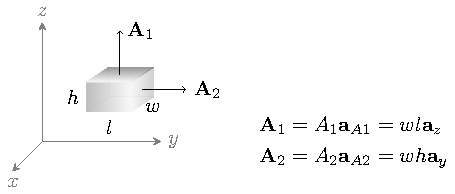
\includegraphics[height=2.5cm]{figBasicFactsVectorArea}
\caption{سمتیہ رقبہ کا تعارف‬}
\label{شکل_حقائق_رقبہ_سمتیہ}
\end{figure}
%
\begin{align*}
A_1&=wl\\
\kvec{a_{A1}}&=\az
\end{align*}
لہٰذا
\begin{align}
\kvec{A_1}=A_1 \kvec{a_{A1}}= w l \az
\end{align}
اسی طرح دائیں جانب سطح \سمتیہ{A_2} سمتیہ  کا طول \عددیء{A_2} ہے اور اس کی سمت \سمتیہ{a_{A2}} ہے۔ یعنی
\begin{align*}
A_2=wh\\
\kvec{a_{A2}}=\ay
\end{align*}
لہٰذا
\begin{align}
\kvec{A_2}=A_2 \kvec{a_{A1}}=w h \ay
\end{align}
یوں نیچے کی سطح کا رقبہ \عددیء{A_3=wl} ہے اور اس کی سمت خلاء کی  اکائی سمتیہ $\az$ کے اُلٹ ہے لہٰذا
\begin{align}
\kvec{A_3}=A_3 \kvec{a_{A3}}=wl (-\az)=-wl \az
\end{align}
یہاں دھیان کریں کہ رقبہ ہر صورت میں مثبت ہی ہوتا ہے البتہ اس کی سمت مثبت یا منفی ہو سکتی ہے۔ یہ بات کسی بھی سمتیہ کے لئے درست ہے لہٰذا کسی بھی سمتیہ کا طول ہر صورت میں مثبت ہی ہوتا ہے البتہ اس کی سمت مثبت یا منفی ہو سکتی ہے۔

\حصہ{رقبہ عمودی تراش}
زاویہ قائمہ بناتے ہوئے لمبائی میں کسی چیز کی کٹائی کو \اصطلاح{عمودی تراش}\فرہنگ{عمودی تراش}\حاشیہب{cross section}\فرہنگ{cross section} کہتے ہیں۔	

شکل \حوالہ{شکل_حقائق_رقبہ_عمودی}  میں ایک سلاخ دکھائی گئی ہے۔ اس کو اکائی سمتیہ $\ay$ کی سمت میں لٹایا گیا ہے۔ اگر ہم تصور میں اس سلاخ کو لمبائی کی عمودی سمت میں کاٹیں تو اس کا جو سرا بنے گا اس سطح کے رقبہ کو \اصطلاح{رقبہ عمودی تراش}\فرہنگ{عمودی تراش!رقبہ}\حاشیہب{cross sectional area} کہتے ہیں۔ شکل میں دکھایا گیا رقبہ عمودی تراش \سمتیہ{A} کی مقدار \عددیء{A} ہے جہاں
\begin{align}
A=wh
\end{align}
مسئلہ کو دیکھتے ہوئے اس رقبہ عمودی تراش کی سمت کا تعین کیا جاتا ہے۔ شکل میں اس کی سمت  \سمتیہ{a_A} خلاء کے اکائی سمتیہ  $\ay$ کی جانب ہے لہٰذا
\begin{align}
\kvec{a_A}=\ay
\end{align}
شکل میں بائیں جانب سلاخ کے نچلے کونے پر اکائی سمتیہ  $\ay$  اور  $\az$ دکھائے گئے ہیں۔ان کے ابتدائی نقطہ پر گول دائرہ میں ایک نقطہ دکھایا گیا ہے۔گول دائرہ میں بند نقطہ صفحہ سے عمودی طور پر کتاب کی باہر جانب سمت کو ظاہر کرتا ہے۔یہاں یہ سمتیہ  $\ax$ کی سمت دکھلا رہا ہے۔اس کی اُلٹ سمت یعنی صفحہ کی عمودی اندر کی جانب کو گول دائرہ میں بند صلیب کے نشان سے ظاہر کیا جاتا ہے۔
%
\begin{figure}
\centering
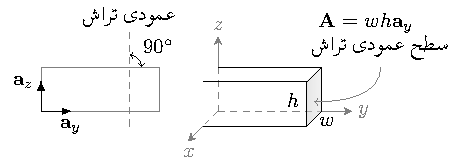
\includegraphics[height=2.5cm]{figBasicFactsCrossSectionalArea}
\caption{رقبہ  عمودی تراش}
\label{شکل_حقائق_رقبہ_عمودی}
\end{figure}
%
\حصہ{برقی میدان اور مقناطیسی میدان}
\جزوحصہ{برقی میدان اور برقی میدان کی شدت}
\اصطلاح{کولمب کے قانون}\فرہنگ{قانون!کولمب}\حاشیہب{Coulomb's law}\فرہنگ{Coulomb's law} کے تحت چارج شدہ جسموں کے درمیان قوت کشش\حاشیہب{attractive force} یا قوت دفع\حاشیہب{repulsive force} ان اجسام پر چارج کی مقدار کے حاصل ضرب کے راست متناسب اور باہمی فاصلہ کے مربع کے بالعکس متناسب ہوتی ہے۔ اس قانون کو مساوات کی شکل میں یوں لکھا جاتا ہے۔
\begin{align}
A=\frac{q_1 q_2}{4 \pi \epsilon r^2}
\end{align}
	اگر ایک چارج کسی جگہ موجود ہو اور دوسرا چارج اس کے قریب لایا جائے تو دوسرے چارج پر کشش یا دفع کی قوت عمل کرے گی جس کا تعین کولمب کے قانون سے ہوتا ہے۔ اگر دوسرے چارج کو پہلے چارج سے آہستہ آہستہ دور لے جائیں تو قوت کشش یا دفع کم ہوتی جاتی ہے۔ ایک خاص فاصلے کے بعد یہ قوت عملی طور پر صفر ہو جاتی ہے اور دوسرا چارج پہلے چارج کے حلقہ اثر سے باہر ہو جاتا ہے۔ اس حلقہ کے اندر واقع جگہ کو \اصطلاح{برقی میدان} کہا جاتا ہے۔ برقی میدان کسی ایک چارج کی وجہ سے بھی ہو سکتا ہے اور بہت سے چارجوں کی وجہ سے بھی ہو سکتا ہے۔ لہٰذا برقی میدان کی تعریف یوں کی جاتی ہے۔

 کسی چارج کے برقی میدان سے مراد چارج کے اِردگرد وہ جگہ ہے جس میں اس کا برقی اثر محسوس کیا جاتا ہے-

	\اصطلاح{برقی میدان کی شدت}\فرہنگ{برقی میدان!شدت}\حاشیہب{electric field intensity}\فرہنگ{electric field!intensity} \سمتیہ{E} کی مقدار اور اس کی سمت کسی مقام پر معلوم کرنے کا طریقہ یہ ہے کہ ایک مثبت اکائی چارج  کو اگر کسی چارج  \عددیء{Q} کے برقی میدان میں رکھا جائے تو جس سمت میں وہ مثبت اکائی چارج حرکت کرے یا حرکت کرنے کے لئے مائل ہو، وہی برقی میدان کی شدت کی سمت ہو گی اور جو قوت اس پر اثر انداز ہو وہ برقی میدان کی شدت ہوگی۔برقی میدان کی شدت کی اکائی \اصطلاح{وولٹ فی میٹر}\حاشیہب{\si{\volt / \meter}} ہے۔

	 کولمب کے قانون یعنی مساوات  کی مدد سے ایک چارج  \عددیء{Q} کی برقی میدان کی شدت کی مقدار یوں حاصل کی جا سکتی ہے۔چارج  \عددیء{Q} اور اکائی چارج یعنی ایک کولمب چارج کے درمیان قوتِ کشش یا قوتِ دفع 
\begin{align}
F=\frac{Q \times 1}{4 \pi \epsilon r^2}=\frac{Q}{4\pi\epsilon r^2}
\end{align}
نیوٹن ہو گی۔یہی برقی میدان کی شدت کی مقدار ہے یعنی
\begin{align}
E=\frac{Q}{4\pi\epsilon r^2}
\end{align}
اگر دو چارجوں کے درمیان سیدھی لکیر کھینچی جائے تو ان کے مابین قوتِ کشش یا قوتِ دفع کی سمت اس لکیر کی سمت میں ہو گی۔

\جزوحصہ{مقناطیسی میدان اور مقناطیسی میدان کی شدت}
\اصطلاح{مقناطیسی میدان} اور \اصطلاح{مقناطیسی میدان کی شدت}\فرہنگ{مقناطیسی میدان!شدت}\حاشیہب{magnetic field intensity}\فرہنگ{magnetic field!intensity} بالکل برقی میدان اور برقی میدان کی شدت کی طرح ہوتی ہے۔

	مقناطیسی میدان کی تعریف یوں کی جاتی ہے۔ کسی مقناطیس کے مقناطیسی میدان سے مراد مقناطیس کے اِردگرد وہ جگہ ہے جس میں اس کا مقناطیسی اثر محسوس کیا جاتا ہے۔

\حصہ{سطحی اور حجمی  کثافت}
\جزوحصہ{سطحی کثافت}
اکائی رقبہ کی سطح پر کسی چیز کی کُل مقدار کو اس چیز کی \اصطلاح{سطحی کثافت}\فرہنگ{سطحی کثافت}\حاشیہب{surface density}\فرہنگ{surface density} کہتے ہیں۔ مثال کے طور پر اگر رقبہ \عددیء{A} پر کسی متغیرہ کی کُل مقدار  \عددیء{\phi} ہو تب اس متغیرہ کی اوسط سطحی کثافت \سیدھازیرنوشت{B}{اوسط}  یہ ہوگی
\begin{align}
B_{\textup{اوسط}}=\frac{\phi}{A}
\end{align}
اس مساوات کو یوں بھی لکھا جا سکتا ہے
\begin{align}
\phi=B_{\textup{اوسط}} A
\end{align}
یعنی اگر ہمیں کسی سطح پر ایک متغیرہ کی اوسط سطحی کثافت معلوم ہو تب ہم اس سطح پر اس متغیرہ کی کُل مقدار اس مساوات کی مدد سے معلوم کر سکتے ہیں۔ 

اگر سطح پر متغیرہ ہر جگہ یکساں نہ ہو تب اس سطح پر سطحی کثافت جگہ جگہ تبدیل ہوگی۔ اس صورت میں اگر اتنا چھوٹا رقبہ لیا جائے کہ اس پر متغیرہ یکساں تصور کیا جا سکے تب اس نقطہ پر سطحی کثافت یوں حاصل ہوگی
\begin{align}
B=\frac{\Delta \phi}{\Delta A}
\end{align}
جہاں \عددیء{\Delta A} یہ چھوٹا رقبہ اور  \عددیء{\Delta \phi} اس پر متغیرہ کی چھوٹی سی مقدار ہے۔ اگر یہ رقبہ ایک نقطہ کی مانند کر دیا جائے تب اس مساوات کو یوں لکھا جائے گا۔
\begin{align}
B=\frac{\dif \phi}{\dif A}
\end{align}
 اس مساوات کو ہم یوں بھی بیان کر سکتے ہیں
\begin{align}
\dif \phi =B \dif A
\end{align}
یعنی اگر ہمیں کسی نقطہ پر ایک متغیرہ کی سطحی کثافت معلوم ہو تب اس نقطہ کے چھوٹے سے رقبہ پر ہم اس متغیرہ کی کم سے کم  کُل مقدار اس مساوات کی مدد سے معلوم کر سکتے ہیں۔

اسی طرح اگر ایک برقی تار کا رقبہ عمودی تراش \عددیء{A} ہو اور اس میں برقی رو \عددیء{I} گزر رہی ہو تو اس تار میں اوسط کثافتِ برقی رو 
\begin{align}
\rho_{\textup{اوسط}}=\frac{I}{A}
\end{align}
ہو گی۔

\حصہ{حجمی کثافت}
  اکائی حجم میں کسی چیز کی کُل مقدار کو اس چیز کی \اصطلاح{حجمی کثافت} کہتے ہیں۔یہاں ہم کمیت کی مثال لیتے ہیں۔ اگر کسی چیز کا حجم \عددیء{V} اور اس کی کمیت \عددیء{m} ہو تب اس کی اوسط حجمی کثافت یہ ہو گی۔
\begin{align}
\rho_{\textup{واسط}}=\frac{m}{V}
\end{align}
اسی طرح اگر اس چیز کی کمیت اس کے حجم میں جگہ جگہ مختلف ہو تب اس کی ایک نقطہ کی حجمی کثافت معلوم کرنے کے لئے اس کا اتنا چھوٹا حصہ لیا جاتا ہے کہ اس چھوٹے حصہ میں اس کی کمیت کو ہر جگہ یکساں تصور کیا جا سکے تب اس چھوٹے حصے کی حجمی کثافت یہ ہوگی۔
\begin{align}
\rho=\frac{\Delta m}{\Delta V}
\end{align}
اب اگر اس چھوٹے حصے کو ایک نقطہ مانند کر دیا جائے تب ہم لکھ سکتے ہیں کہ
\begin{align}
\rho=\frac{\dif m}{\dif V}
\end{align}
اور
\begin{align}
\dif m=\rho \dif V
\end{align}
یعنی اگر ہمیں ایک نقطہ کی حجمی کثافت معلوم ہو تب ہم ایک نہایت چھوٹے حجم کی کمیت اس مساوات کی مدد سے حاصل کر سکتے ہیں۔

\حصہ{ضربِ صلیبی اور ضربِ نقطہ}
دو مقداری متغیرات کا حاصلِ ضرب مقداری متغیرہ ہی ہوتی ہے جبکہ دو سمتیہ متغیرات کا حاصلِ ضرب سمتیہ متغیرہ یا مقداری متغیرہ ہو سکتی ہے۔ان دو اقسام کے ضرب پر یہاں غور کیا جائے گا۔
\جزوحصہ{ضرب صلیبی}
ایسی دو سمتیہ متغیرات کا ضرب جس کا حاصلِ ضرب سمتیہ متغیرہ ہو کو ضربِ صلیبی کہتے ہیں اور اسے یوں لکھا جاتا ہے۔
\begin{align}
\kvec{C}=\kvec{A} \times \kvec{B}
\end{align}
ضربِ صلیبی میں ضرب کے نشان کو صلیب کی علامت سے ظاہر کیا جاتا ہے۔اسی سے اس کا نام ضربِ صلیبی لیا گیا ہے۔

حاصل ضرب سمتیہ \سمتیہ{C} کی مقدار
\begin{gather}
\begin{aligned}
C=\abs{\kvec{C}} &= \abs {\kvec{A}} \abs{\kvec{B}} \sin \theta_{AB}\\
&=A B \sin \theta_{AB}
\end{aligned}
\end{gather}
ہے جہاں \عددیء{\theta_{AB}} ان کے مابین زاویہ ہے۔اس حاصل سمتیہ کی سمت دائیں ہاتھ  کے قانون سے یوں حاصل کی جاتی ہے۔ 

اگر آپ دائیں ہاتھ کی چار انگلیوں کو سمتیہ \سمتیہ{A} کی سمت میں رکھ کر \سمتیہ{B} سمتیہ کی سمت موڑیں تو اس ہاتھ کا انگوٹھا \سمتیہ{C}  سمتیہ کی سمت کو ظاہر کرے گا۔

\ابتدا{مثال}
مندرجہ ذیل ضرب صلیبی حاصل کریں۔
\begin{itemize}
\item
$\ax \times \ay \quad \ay \times \az \quad \az \times \ax \quad \ax \times \az$ \\
\item
 $\az \times \ay \quad \ay \times \ay \quad \arho \times \atheta \quad \az \times \arho$
\end{itemize}

حل: اس مثال میں سب سمتیہ اکائی ہیں۔اکائی سمتیہ کا طول ایک کے برابر ہوتا ہے۔ لہٰذا
\begin{itemize}
\item
$\ax \times \ay=(1)(1) \sin 90 \az =\az$\\
\item
$\ay \times \az=(1)(1) \sin 90 \ax =\ax$\\
\item
$\az \times \ax=(1)(1) \sin 90 \ay =\ay$\\
\item
$\ax \times \az=(1)(1) \sin 90 (-\ay) =-\ay$\\
\item
$\az \times \ay=(1)(1) \sin 90 (-\ax) =-\ax$\\
\item
اس مثال میں چونکہ دونوں سمتیہ ایک ہی جانب ہیں لہٰذا ان کے مابین زاویہ صفر ہے۔صفر زاویہ کا سائن صفر ہی ہوتا ہے یعنی \عددیء{\sin 0 =0} لہٰذا ان دو سمتیہ کا ضربِ صلیبی صفر ہو گا\\
$\ay \times \ay=(1)(1) \sin 0  =0$\\
\item
$\arho \times \atheta=(1)(1) \sin 90  \az =\az$\\
\item
$\az \times \arho=(1)(1) \sin 90 \atheta =\atheta $\\
\end{itemize}
\انتہا{مثال}
%
\ابتدا{مثال}
شکل \حوالہ{شکل_حقائق_کارتیسی_مروڑ_کا_حل} میں  چار نیوٹن کی قوت \سمتیہ{F} محور سے تین میٹر کی سمتیہ فاصلہ \سمتیہ{L}  پر لاگو ہے۔اسی شکل میں اس کی تفصیل دی گئی ہے۔اس قوت کی مروڑ  حاصل کریں۔
	حل:
	مروڑ \سمتیہ{T} کی تعریف یہ ہے
\begin{align}
\kvec{T}=\kvec{L} \times \kvec{F}
\end{align}
کارتیسی نظام میں اس سمتیہ فاصلہ کو یوں لکھا جا سکتا ہے
\begin{align}
\kvec{L}=L \sin \theta \ax-L \cos \theta \ay
\end{align}
لہٰذا
\begin{align*}
\kvec{T}&=\left(L \sin \theta \ax-L \cos \theta \ay \right) \times F \ay\\
&=L \sin \theta \ax \times F \ay-L \cos \theta \ay \times F \ay\\
&= L F \sin \theta \az
\end{align*} 
یہاں پچھلی مثال کی مدد سے \عددیء{\ax \times \ay=\az} اور \عددیء{\ay \times \ay=0} لی گئی ہیں۔یوں
\begin{align*}
\kvec{T}= L F \sin \theta \az=12 \sin \theta \az \quad \si{\newton \meter}
\end{align*}
ہے۔اس مثال میں \عددیء{\theta_{LF}=180\degree-\theta} ہے۔چونکہ کسی بھی زاویہ \عددیء{\alpha}   کے لئے \عددیء{\sin \alpha=\sin(180\degree-\alpha)} ہوتا ہے لہٰذا اس مروڑ کو یوں بھی لکھا جا سکتا ہے۔
\begin{align*}
\kvec{T}&=LF\sin \theta \az\\
&=L F \sin \theta_{LF}\az
\end{align*}
یہی جواب ضربِ صلیبی کی تعریف یعنی مساوات اور دائیں ہاتھ کے قانون کی مدد سے زیادہ آسانی سے حاصل ہوتا ہے۔
\انتہا{مثال}
%
\begin{figure}
\centering
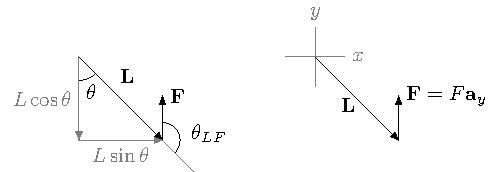
\includegraphics[height=2.5cm]{figBasicFactsVectorCrossProduct}
\caption{کارتیسی نظام میں مروڑ کا حل}
\label{شکل_حقائق_کارتیسی_مروڑ_کا_حل}
\end{figure}
%
\جزوحصہ{ضربِ نقطہ}
ایسی دو سمتیہ متغیرات کا ضرب جس کا حاصلِ ضرب مقداری متغیرہ ہو کو ضربِ نقطہ کہتے ہیں اور اسے یوں لکھا جاتا ہے۔
\begin{align}
\kvec{C}=\kvec{A} \cdot \kvec{B}
\end{align}
ضربِ نقطہ میں ضرب کے نشان کو نقطہ کی علامت سے ظاہر کیا جاتا ہے۔اسی سے اس کا نام ضربِ نقطہ لیا گیا ہے۔

ضربِ نقطہ میں حاصلِ ضرب مقداری کی مقدار یوں حاصل ہوتی ہے
\begin{gather}
\begin{aligned}
\kvec{C}&=\kvec{A} \cdot \kvec{B}\\
&=\abs{\kvec{A}} \abs{\kvec{B}} \cos \theta_{AB}\\
&=A B \cos \theta_{AB}
\end{aligned}
\end{gather}
جہاں \عددیء{\theta_{AB}} ان دو کے مابین زاویہ ہے۔

\ابتدا{مثال}
مندرجہ ذیل ضربِ نقطہ حاصل کریں
\begin{itemize}
\item
$\ax \cdot \ax \quad \ay \cdot \ay \quad \az \cdot \az$\\
\item
$\ax \cdot \ay \quad \ay \cdot \az \quad \arho \cdot \arho \quad \arho \cdot \atheta$
\end{itemize}

حل:اس مثال میں سب اکائی سمتیہ ہیں۔اکائی سمتیہ کا طول ایک کے برابر ہوتا ہے۔
\begin{itemize}
\item
$\ax \cdot \ax =(1) (1) \cos 0=1$\\
\item
$\ay \cdot \ay =(1) (1) \cos 0=1$\\
\item
$\az \cdot \az =(1) (1) \cos 0=1$\\
\item
$\ax \cdot \ay =(1) (1) \cos 90\degree=0$\\
\item
$\ay \cdot \az =(1) (1) \cos 90\degree=0$\\
\item
$\arho \cdot \arho =(1) (1) \cos 0=1$\\
\item
$\arho \cdot \atheta =(1) (1) \cos 90\degree=0$\\
\end{itemize}
\انتہا{مثال}
%
\ابتدا{مثال}
شکل \حوالہ{شکل_حقائق_کارتیسی_کام}  میں قوت \سمتیہ{F} ایک بار کو دھکیل رہی ہے۔سمتیہ فاصلہ  \سمتیہ{L} طے کرنے پر قوت کتنا کام کر چکی ہو گی۔

	حل:
	کام  \عددیء{W} کی تعریف یہ ہے
\begin{align}
W=\kvec{F} \cdot \kvec{L}
\end{align}
ہم کارتیسی نظام میں سمتیہ فاصلہ کو یوں لکھ سکتے ہیں
\begin{align}
\kvec{L}=L \cos \theta_{FL} \ax +L \sin \theta_{FL} \ay
\end{align}
لہٰذا
\begin{gather}
\begin{aligned}
W &= (F \ax) \cdot (L \cos \theta_{FL} \ax +L \sin \theta_{FL} \ay)\\
&=F L \cos \theta_{FL} (\ax \cdot \ax)+ F L \sin \theta_{FL} (\ax \cdot \ay)\\
&= F L \cos \theta_{FL}
\end{aligned}
\end{gather}
%
\begin{figure}
\centering
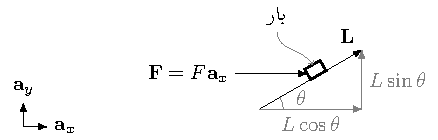
\includegraphics[height=2.5cm]{figBasicFactsWorkAsDotProduct}
\caption{کارتیسی نظام میں کام}
\label{شکل_حقائق_کارتیسی_کام}
\end{figure}
جہاں پچھلی مثال کی مدد سے \عددیء{\ax \cdot \ax=1} اور \عددیء{\ax \cdot \ay=0} لی گئی ہیں۔ یہی جواب ضربِ نقطہ کی تعریف یعنی مساوات سے با آسانی حاصل ہوتا ہے۔
\انتہا{مثال}
%
\حصہ{تفرق  اور جُزوی تفرق}
مساوات میں ایک تفاعل جس میں مقررہ ہے کا تفرق دیا گیا ہے جبکہ مساوات  میں ایک تفاعل کا جُزوی تفرق  دیا گیا ہے۔
\begin{gather}
\begin{aligned}
B (\theta )&=B_0 \cos \theta\\
\frac{\dif B}{\dif \theta}&=-B_0 \sin \theta
\end{aligned}
\end{gather} 
%
\begin{align}
\partial W(x,\lambda)=\frac{\partial W}{\partial x} \dif x+\frac{\partial W}{\partial \lambda} \dif \lambda
\end{align}

\حصہ{خطی تکمل}
مساوات  میں ایک تفاعل \عددیء{B(\theta)} دیا گیا ہے جسے شکل \حوالہ{شکل_حقائق_کوسائن_موج}  میں دکھایا گیا ہے۔ اس کی طولِ موج  \عددیء{2 \pi} ریڈیئن کے برابر ہے۔ ہم \عددیء{-\pi/2<\theta<\pi/2} کے مابین اس کا اوسط معلوم کرتے ہیں۔ یہ تکمل سے یوں ہو گا۔
\begin{align}
B(\theta)=B_0 \cos \theta
\end{align}
%
\begin{align}
B_{\textup{اوسط}}=\frac{B_0}{\pi}\int_{-\frac{\pi}{2}}^{\frac{\pi}{2}} \cos \theta \dif \theta=\frac{2 B_0}{\pi}
\end{align}
اسی طرح اگر اسی خطہ پر تفاعل کے مربع یعنی \عددیء{B^2}  کا اوسط درکار ہو تو ایسا کرنا مساوات میں دکھایا گیا ہے۔
\begin{gather}
\begin{aligned}
B^2_{\textup{اوسط}}&=\frac{B_0^2}{\pi}\int_{-\frac{\pi}{2}}^{\frac{\pi}{2}} \cos^2 \theta \dif \theta\\
&=\frac{B_0^2}{\pi}\int_{-\frac{\pi}{2}}^{\frac{\pi}{2}}\frac{1+\cos 2 \theta}{2} \dif \theta\\
&=\frac{B_0^2}{2}
\end{aligned}
\end{gather}
تفاعل کے مربع کی اوسط کا جزر  بہت اہمیت رکھتا ہے۔لہٰذا اس تفاعل کے مربع کی اوسط کا جزر \عددیء{B_{rms}} مساوات  کی مدد سے یوں حاصل ہوتا ہے۔
\begin{align}
B_{rms}=\sqrt{B^2_{\textup{اوسط}}}=\frac{B_0}{\sqrt{2}}
\end{align}
یہ ایک بہت اہم نتیجہ ہے جو آپ کو زبانی یاد ہونا چاہئے۔ یہ مساوات ہر سائن نما تفاعل کے لئے درست ہے۔کسی بھی متغیرہ کے مربع کی اوسط کا جزر اس متغیرہ کا موثر قیمت کہلاتا ہے۔
%
\begin{figure}
\centering
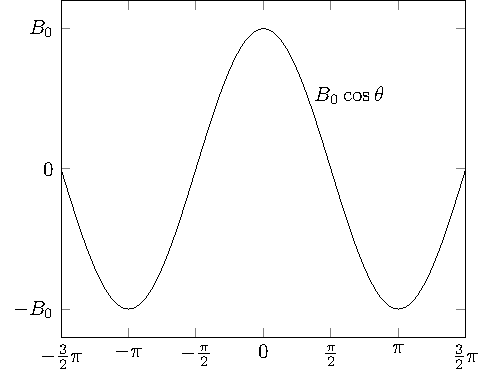
\includegraphics{figBasicFactsCosineWave}
\caption{کوسائن موج}
\label{شکل_حقائق_کوسائن_موج}
\end{figure}
\حصہ{سطحی تکمل}
مثال کے طور پر اگر مساوات  شکل  \حوالہ{شکل_حقائق_نلکی_سطحی_تکمل} میں نلی کے بیرونی سطح پر متغیرہ \عددیء{B} کی مقدار بتلاتی ہے اور یہ متغیرہ سطحی کثافت کو ظاہر کرے  ہم آدھے بیرونی سطح مثلاً زاویہ \عددیء{-\pi/2} اور \عددیء{\pi/2} کے مابین اس کی کُل مقدار \عددیء{\phi} معلوم کرتے ہیں۔اس سطح میں نلی کے دونوں سرے شامل نہیں ہیں۔

	ہم نلی کے بیرونی سطح پر رقبہ  \عددیء{\Delta A} لیتے ہیں جس کی قوسِ صغیرہ \عددیء{\rho \Delta\theta}  اور لمبائی \عددیء{l} ہے۔یہ سطح \عددیء{abcd} ہے۔\عددیء{\Delta \theta} کو نہایت کم کرتے ہوئے سطح کا رقبہ \عددیء{\rho l \dif \theta} لکھا جا سکتا ہے۔چونکہ اس سطح پر \عددیء{B} کی مقدار محوری لمبائی  کی جانب تبدیل نہیں ہو رہی اس لئے سطح \عددیء{\Delta A}  پر \عددیء{\Delta \phi=B \Delta A} ہو گا اور کُل \عددیء{\phi} تکمل کی مدد سے یوں حاصل ہو گا۔
\begin{figure}
\centering
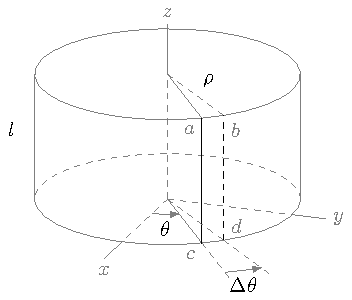
\includegraphics{figBasicFactsCylindricalSurfaceIntegral}
\caption{نلی کی بیرونی سطح پر متغیرہ کا تکمل کُل مقدار دے گی۔}
\label{شکل_حقائق_نلکی_سطحی_تکمل}
\end{figure}
%
\begin{align}
\Delta \phi=B \Delta A=B_0 l \rho \cos \theta \dif \theta
\end{align}
%
\begin{align}
\phi = B_0 l \rho \int_{-\pi/2}^{\pi/2} \cos \theta \dif \theta =2 B_0 l \rho
\end{align}
اب ہم یہی مقدار نلی کے آدھے بیرونی سطح پر کہیں پر بھی حاصل کرنا چاہیں تو ہمیں صرف تکمل کے دو حد تبدیل کرنے ہوں گے۔  اگر ہم مساوات  میں نچلا حد \عددیء{(-\pi/2-\alpha)} اور اُوپر کا حد \عددیء{(\pi/2-\alpha)} لیں تو یہ حاصل ہوگا۔
\begin{align}
\phi (\alpha) = B_0 l \rho \int_{-\frac{\pi}{2}-\alpha}^{\frac{\pi}{2}-\alpha} \cos \theta \dif \theta =2 B_0 l \rho \cos \alpha
\end{align}
یہاں  \عددیء{\phi(\alpha)} اس بات کو واضح کرتا ہے کہ نتیجہ \عددیء{\alpha} پر منحصر ہے۔ یہ ایک بہت اہم مساوات ہے۔ مساوات میں  اگر \عددیء{\alpha=0} ہو تو مساوات   ملتا ہے۔

\حصہ{ دوری سمتیہ}
\begin{figure}
\centering
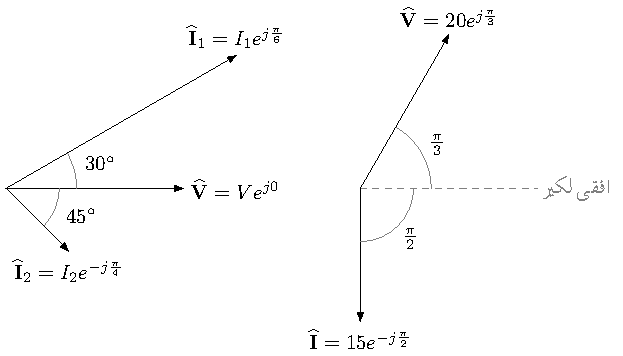
\includegraphics{figBasicFactsPhasors}
\caption{دوری سمتیہ}
\label{شکل_حقائق_دوری_سمتیات}
\end{figure}
سائن نما موج جن کا تعدد معین ہو کو دوری سمتیہ سے ظاہر کرنا نہایت مفید ثابت ہوتا ہے۔ مساواتِ یولر
\begin{align}
A_0 e^{\mp j (\omega t + \phi)}=A_0 \cos (\omega t +\phi) \mp j \sin (\omega t+\phi)
\end{align}
کی مدد سے کو-سائن موج یوں لکھی جا سکتی ہے
\begin{align}
A_0 \cos (\omega t +\phi)=\frac{A_0}{2} \left(e^{j(\omega t +\phi)} -e^{-j(\omega t +\phi)}\right)
\end{align}
اس سے ثابت ہوتا ہے کہ کو-سائن موج دراصل دو مخلوط اعداد کا مجموعہ ہے۔ مساواتِ یولر ایک مخلوط عدد کو ظاہر کرتا ہے جس کے دو جُز ہیں۔ اس کا ایک جُز حقیقی عدد ہے اور اس کا دوسرا جُز فرضی عدد ہے۔اس کا حقیقی جُز کو-سائن موج کو ظاہر کرتا ہے۔ لہٰذا ایک کو-سائن موج  \عددیء{A_0 e^{j(\omega t +\phi)}} یا \عددیء{A_0 e^{-j(\omega t +\phi)}} کا حقیقی جُز ہوتا ہے۔ رسمی طور پر سائن نما موج کو \عددیء{A_0 e^{j(\omega t +\phi)}} سے ظاہر کیا جاتا ہے۔ مزید یہ کہ اس عدد کو چھوٹا کر کے صرف \عددیء{A_0 e^{j\phi}} یا پھر \عددیء{A_0 \phase{\phi}} لکھا جاتا ہے۔کو-سائن موج کے اس طرح ظاہر کرنے کو دوری سمتیہ کہتے ہیں جہاں اس سمتیہ کا طول \عددیء{A_0} اور اُفقی لکیر سے زاویہ \عددیء{\phi} ہے۔

	 دوری سمتیہ استعمال کرتے وقت آپ کو یہ ذہن میں رکھنا ہوتا ہے کہ یہ ایک کو-سائن موج ہے جس کا حیطہ  \عددیء{A_0} ، دوری زاویہ \عددیء{\phi} اور زاویاتی تعدد \عددیء{\omega} ہے۔

اس کتاب میں دوری سمتیہ کو سادہ طرزِ لکھائی میں انگریزی کے بڑے حروف جن پر ٹوپی کا نشان ہو سے ظاہر کیا جائے گا، یعنی \عددیء{\hat{I},\hat{V}}  وغیرہ اور ان کے طول کو بغیر ٹوپی کے نشان کے اسی حرف سے ظاہر کیا جائے گا۔مثلاً برقی دباؤ \عددیء{v= 20 \cos (\omega t +\frac{\pi}{3})} کے لئے یہ سب درست ہیں۔
\begin{gather}
\begin{aligned}
v&=20 \cos (\omega t +\frac{\pi}{3})\\
\hat{V}&=20 e^{j \frac{\pi}{3}}\\
\hat{V}&=20 \phase{\frac{\pi}{3}}\\
V&=20
\end{aligned}
\end{gather}
اس مساوات میں پہلا جُز ایک عام کوسائن موج ہے۔ دوسرا جُز اِسی کو دوری سمتیہ سے ظاہر کر رہا ہے۔ تیسرا اس دوری سمتیہ کا طول اور چوتھا اس کا زاویہ بتلا رہا ہے۔
\begin{figure}
\centering
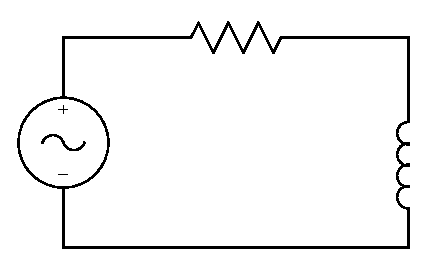
\includegraphics{figBasicFactsRLcircuit}
\caption{دوری سمتیہ کی مدد سے \عددیء{RL} دور کا حل۔}
\label{شکل_حقائق_دوری_سمتیہ_سے_دور_حل}
\end{figure}
	دوری سمتیہ کو عام سمتیوں کی طرح ہی تصور کیا جاتا ہے۔ اس مساوات میں \عددیء{\hat{V}} کا طول \عددیء{20} اور اُفقی لکیر سے زاویہ  \عددیء{\tfrac{\pi}{3}} ریڈیئن ہے۔زاویہ اُفقی لکیر سے گھڑی کی اُلٹی سمت ناپا جاتا ہے۔ اس سمت میں زاویہ مثبت ہے۔ شکل \حوالہ{شکل_حقائق_دوری_سمتیات} میں اسے اور چند اور دوری سمتیہ دکھائے گئے ہیں۔

برقی دور حل کرتے وقت برقی دباؤ \عددیء{\hat{V}} کو اُفقی سمت میں بنا کر برقی رو  \عددیء{\hat{I}} اس کی نسبت سے بنایا جاتا ہے۔شکل \حوالہ{شکل_حقائق_دوری_سمتیات}   میں \عددیء{\hat{I_1}} تیس درجہ زاویہ برقی دباؤ سے آگے  ہے جبکہ  \عددیء{\hat{I_2}}  پینتالیس درجہ زاویہ اس کے پیچھے  ہے۔یہاں یہ دھیان رہے کہ شکل میں  \عددیء{45\degree} مثبت لکھا گیا ہے۔چونکہ یہ اُفقی لکیر سے زاویہ ناپنے کی اُلٹ سمت میں ہے لہٰذا یہ ایک منفی زاویہ ہے۔

یہاں دوری سمتیوں کو استعمال کر کے ایک سادہ برقی دور حل کرتے ہیں۔ یوں ان سے وابستگی پیدا ہو جائے گی اور ان کا استعمال بھی سیکھ لیں گے۔

شکل   ایک سادہ \عددیء{R-L} برقی دور ہے جس پر لاگو برقی دباؤ
\begin{gather}
\begin{aligned}
v(t)&=V_0 \cos (\omega t +\alpha)\\
\hat{V}&=V_0 \phase{\alpha}
\end{aligned}
\end{gather}
ہے۔دوری سمتیہ کے استعمال سے ہم اس میں برقی رو \عددیء{i(t)} معلوم کرنا چاہتے ہیں۔
\begin{gather}
\begin{aligned}
\hat{I}&=\frac{\hat{V}}{R+j X}=\frac{V_0 \phase{\alpha}}{\abs{Z} \phase {\phi_Z}}\\
&=\frac{V_0}{\abs{Z}} \phase{\alpha-\phi_Z}=I_0 \phase{\alpha-\phi_Z}
\end{aligned}
\end{gather}
جہاں \عددیء{\phi_Z} مقاومت کا زاویہ  ہے۔لہٰذا
\begin{align}
i(t)=I_0 \cos (\omega t +\alpha-\phi_Z)
\end{align}

